\chapter{Máquinas de Estado Finito(MEF)}

Una MEF $M$ es una séxtupla $M=(S,I,O,f,g,s^*)$ donde:

\begin{itemize}
\item $S$: Segmento de estado, $s\not=\phi$.
\item $I$: Alfabeto de entrada.
\item $O$: Alfabeto de salida.
\item $s^*$: Estado inicial , $s^*\in S$.
\item $f$: Función de estado siguiente. $f:S\times I \rightarrow S$.
\item $g$: Función de salida. $g:S\times I \rightarrow O$.
\end{itemize}

$$ f(\uplegend{s}{estado actual},\downlegend{x}{simbolo})=\uplegend{s_2}{siguiente estado}$$ %s estado actual, x simbolo, s2 siguiente estado
\subsection{Tipo de Representación}
Existen 2 tipos de representaciones que son las siguientes:

\begin{enumerate}
\item \textbf{Tablas de Estado: }Conocidas como tablas de transmisión. Podemos representar a las MEF $M$ por medio de una tabla que liste.

$f(s,x);g(s,x)\qquad \forall s\in S, \forall x\in I$

\textbf{Ejemplo: }Sea la MEF $M$ donde:

$S=\{ s_0,s_1,s_2\}$

$I=\{0,1\}=Q$

$f$ y $g$ están dados en la siguiente tabla:

\begin{center}
$\begin{array}{c|c|c|c|c}
S/I		&\multicolumn{2}{c}{f}	&\multicolumn{2}{c}{g}\\ 
		&0		&1		&0	&1	\\ \hline
s_0	&s_0	&s_1	&0	&0	\\ \hline
s_1	&s_2	&s_1	&0	&0	\\ \hline
s_2	&s_0	&s_1	&0	&1
\end{array}$
\end{center}

Se pide:
	\begin{itemize}
	\item Obtener $f(s_1,1)$ y $g(s_1,1)$.
	\item Si tenemos como entrada la cadena $u=1010$, determine la cadena de salida $w$.
	
	\textbf{Solución: }
	\item $f(s_1,1)=s_1\qquad g(s_1,1)=0$
	\item Tenemos: $s^*=s_0$, $u=1010$
	\begin{center}
	$\begin{array}{c|c|c|c|c|c}
	Estado	&s_0	&s_1	&s_2	&s_1	&s_2	\\ \hline
	Entrada	&1	&0	&1	&0	&	\\ \hline
	Salida	&0	&0	&1	&0	&	
	\end{array}$\\	
	\end{center}
	$g(s_0,1)=0 \quad f(s_0,1)=s_1 \quad f(s_2,1)=s_1$ %donde g es (3,2), f=(1,3) 
	
	La cadena de salida es $w=0010$.
	\end{itemize}
\item \textbf{Diagramas de Estados: }
	\begin{itemize}
	\item Cada estado interno de $S$ es representado con un nodo.
	\item Dados los estados $s_i,s_j$
	
	si: $\begin{array}{cl}
	f(s_i,x)=s_j	&\mbox{para }x\in I	\\
	g(s_i,x)=y		&y\in O	
	\end{array}$
	\end{itemize}
	Los representamos mediante una arista dirigida desde $s_i$ a $s_j$ y rotulando el arco con la entrada $x$ y la salida $y$
	%grafico: circulo(s_i) flecha(x,y) circulo(s_j)
	\begin{figure}[h]
	\centering
	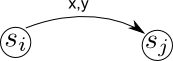
\includegraphics[width=0.3\textwidth]{img_7_1.png} 
	\caption{Representación Diagrama de Estados}
	\end{figure}
	
	Usando el ejemplo anterior, dibujamos el diagrama de estados para $M$.
	%grafico:
	\begin{figure}[h]
	\centering
	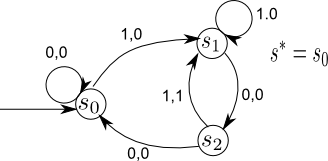
\includegraphics[width=0.5\textwidth]{img_7_2.png} 
	\caption{Diagrama de Estado de $M$}
	\end{figure} 
\end{enumerate}

\section{Sumador Binario}

Sean las cadenas $x,y$

$x=x_5x_4x_3x_2x_1=00111$

$y=x_5y_4y_3y_2y_1=01101$

Un sumador binario en serie es una MEF que nos sirve para hallar x+y.

\textbf{Representación}

%grafico caja
\begin{figure}
\centering
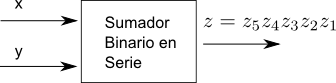
\includegraphics[width=0.5\textwidth]{img_7_3.png} 
\caption{Sumador Binario}
\end{figure}

Para la adición $z=x+y$ tenemos:

$\begin{array}{cccccc}
x=	&0	&0	&1	&1	&1	\\
y=	&0	&1	&1	&0	&1	\\ \hline
	&1	&0	&1	&0	&0
\end{array}$

Podemos modelar este sumador binario mediante una MEF $M$, en la cual.

$S=\{s_0,s_1\}	\qquad \begin{matrix}
s_0 \mbox{ indica un caracter de 0} \\
s_1 \mbox{ indica un caracter de 1}
\end{matrix}$\\

$I=\{00,01,10,11\} \qquad s^*=s_0$

$O=\{0,1\}$

Las funciones $f$ y $g$ quedan definidas en la tabla.

\begin{center}
$\begin{array}{c|cccc|cccc}
S/I	&\multicolumn{4}{c}{f}	&\multicolumn{4}{c}{g}\\
	&00	&01	&10	&11	&00	&01	&10	&11	\\ \hline
s_0	&s_0&s_0&s_0&s_1&0	&1	&1	&0	\\
s_1	&s_0&s_1&s_1&s_1&1	&0	&0	&1
\end{array}$
\end{center}

$$f(s_0,11)=s_1 \qquad g(s_0,11)=0$$

El diagrama de estados para $M$ será (Figura \ref{fig7_4}):

%grafico
\begin{figure}[h]
\centering
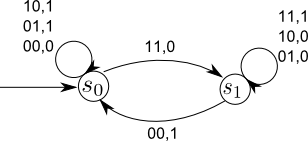
\includegraphics[width=0.5\textwidth]{img_7_4.png} 
\caption{Diagrama de Estados de $M$}\label{fig7_4}
\end{figure}

\textbf{Ejercicio: }Sea $M=(S,I,O,f,g,s^*)$ donde:

$\begin{array}{l}
S=\{s_0,s_1,s_2,s_3\}\\
I=\{a,b,c\} \\
O=\{0,1\}
\end{array}$
\begin{center}
$\begin{array}{c|ccc|ccc}
S/I	&	&f	&	&	&g	&	\\
	&a	&b	&c	&a	&b	&c	\\ \hline
s_0	&s_0&s_3&s_2&0	&1	&1	\\
s_1	&s_1&s_1&s_3&0	&0	&1	\\
s_2	&s_1&s_1&s_3&1	&1	&0	\\
s_3	&s_2&s_3&s_0&1	&0	&1
\end{array}$
\end{center}
Si $s^*=s_0$

\begin{itemize}
\item Obtener la cadena de salida si la entrada es $u=abbccc$.
\item Dibuje el diagrama de estados.
\end{itemize}

\textbf{Solución: }
\begin{center}
$\begin{array}{c|c|c|c|c|c|c}
Estado &s_0	&s_0	&s_3	&s_3	&s_0	&s_2	\\ \hline
Entrada	&a	&b	&b	&c	&c	&c	\\ \hline
Salida	&0	&1	&0	&1	&1	&1
\end{array}$
\end{center}
\begin{align*}
u=abbccc \\
v=101010
\end{align*}

%grafico
\begin{figure}[h]
\centering
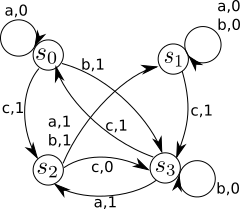
\includegraphics[width=0.4\textwidth]{img_7_5.png}
\caption{Diagrama de Estados}
\end{figure}

\section{Extensión de las funciones $f$ y $g$}

Para una MEF $M=(S,I,O,f,g,s^*)$, la entrada puede ser realizada con un elemento de $I^*$, con la salida $O^*$. Extendemos los dominios de $f$ y $g$ de $S\times I$ a $S\times I^*$.

Para $g$, ampliamos el codominio de $O$ a $O^*$. Con estas extensiones, si $x_1,x_2,x_3...x_k \in I^*$ entonces empezando en cualquier estado $s_1 \in S$ tenemos:
\begin{align*}
f(s_1,x_1)&=s_2	\\
f(s_1,x_1x_2)&=f(f(s_1,s_1),x_2)=f(s_2,x_2)	\\
f(s_1,x_1x_2x_3)&=f(f(\underbrace{f(s_1,x_1)}_{s_2},x_2),x_3)	\\
	&=f(\underbrace{f(s_2,x_2)}_{s_3},x_3)=f(s_3,x_3)	\\
&\vdots	\\
f(s_1,x_1...x_k)&=f(s_k,x_k)=s_{k+1}
\end{align*}

función de estado siguiente extendida.
\begin{align*}
g(s_1,x_1)&=y_1\\
g(s_1,x_1x_2)&=g(s_1,x_1).g(f(s_1,x_1),x_2)\\
&=y_1.g(s_2,x_2)=y_1.y_2\\
g(s_1,x_1x_2x_3)&=g(s_1,x_1).g(s_2,x_2).g(s_3,x_3)\\
&=y_1.y_2.y_3\\
&\vdots\\
g(s_1,x_1...x_k)&=g(s_1,x_1)g(s_2,x_2)...g(s_k,x_k)\\
&=y_1y_2...y_k
\end{align*}

También $f(s_i,\varepsilon)=s_i \qquad \forall s_i \in S$